


\documentclass[a4paper,10pt]{article}
\usepackage{listings,color,epsfig,amsmath,url}
\definecolor{codecolor}{rgb}{0.99,0.97,0.94} % color values Red, Green, Blue
\definecolor{commentcolor}{rgb}{0.1,0.5,0.1} % color values Red, Green, Blue
\definecolor{stringcolor}{rgb}{0.3,0.1,0.1} % color values Red, Green, Blue
\newcommand{\Code}[1]{\texttt{#1} }
\newcommand{\code}[1]{\Code{#1} }
\newcommand{\DB}   {\code{{MOOSDB}}}
\newcommand{\MA}   {\code{{MOOSApp}}}
\newcommand{\Ignore}[1]   {}



\lstset{ frame = shadowbox,
 %language=[Visual]{c++},
 rulesepcolor=\color{black},
 basicstyle=\small } \lstset{
backgroundcolor=\color{codecolor},
keywordstyle=\color{blue}\bfseries,
commentstyle=\color{commentcolor},
stringstyle=\color{stringcolor}\ttfamily, linewidth =
1.2\linewidth,
breaklines=true} %

\lstset{language=C++}
% Title Page
\title{Building and Linking Against MOOS}
\author{Paul Newman}


\begin{document}
\maketitle

\begin{center}
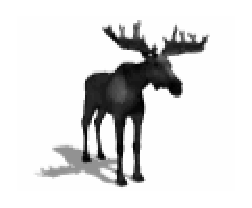
\epsfig{file=images/moose6.eps,width = 0.2\linewidth}
\end{center}
\begin{abstract}
This document will tell you how to build the MOOS project and how to link your own
applications against the MOOS libraries.
\end{abstract}





\section{Introduction}\label{Sec:CompilingAndLinking}
In this document, we'll cover how to compile and link your MOOS Applications.
The simplest way to do this is by using CMake and adding your own source tree as a sibling of the ``Core'' directory
under the MOOS -- this is described in detail in Section \ref{Sec:UsingCMake}. However you may not want to do this,
preferring to handcraft your own  Make files for each platform your application will be running on -- the information you will require to do this is described in Section \ref{Sec:RollYourOwn}.

\subsection{Downloading the Source Tree}

The \code{MOOS} can  be downloaded from \url{http://www.robots.ox.ac.uk/~pnewman/TheMOOS} and also via \code{svn}\footnote{Directions on how to use svn to grab releases can be found on \url{http://www.robots.ox.ac.uk/~pnewman/TheMOOS}.}.

All of the latest MOOS code is cross-platform. Built into
the source tree is a cross-platform build system that relies on
\code{CMake} -- a third-party executable available from
{\it{www.cmake.org}} or the MOOS website.

\section{The Source Tree Shape}

\begin{figure}[ht!]\label{Fig:MOOSTree}
\centering 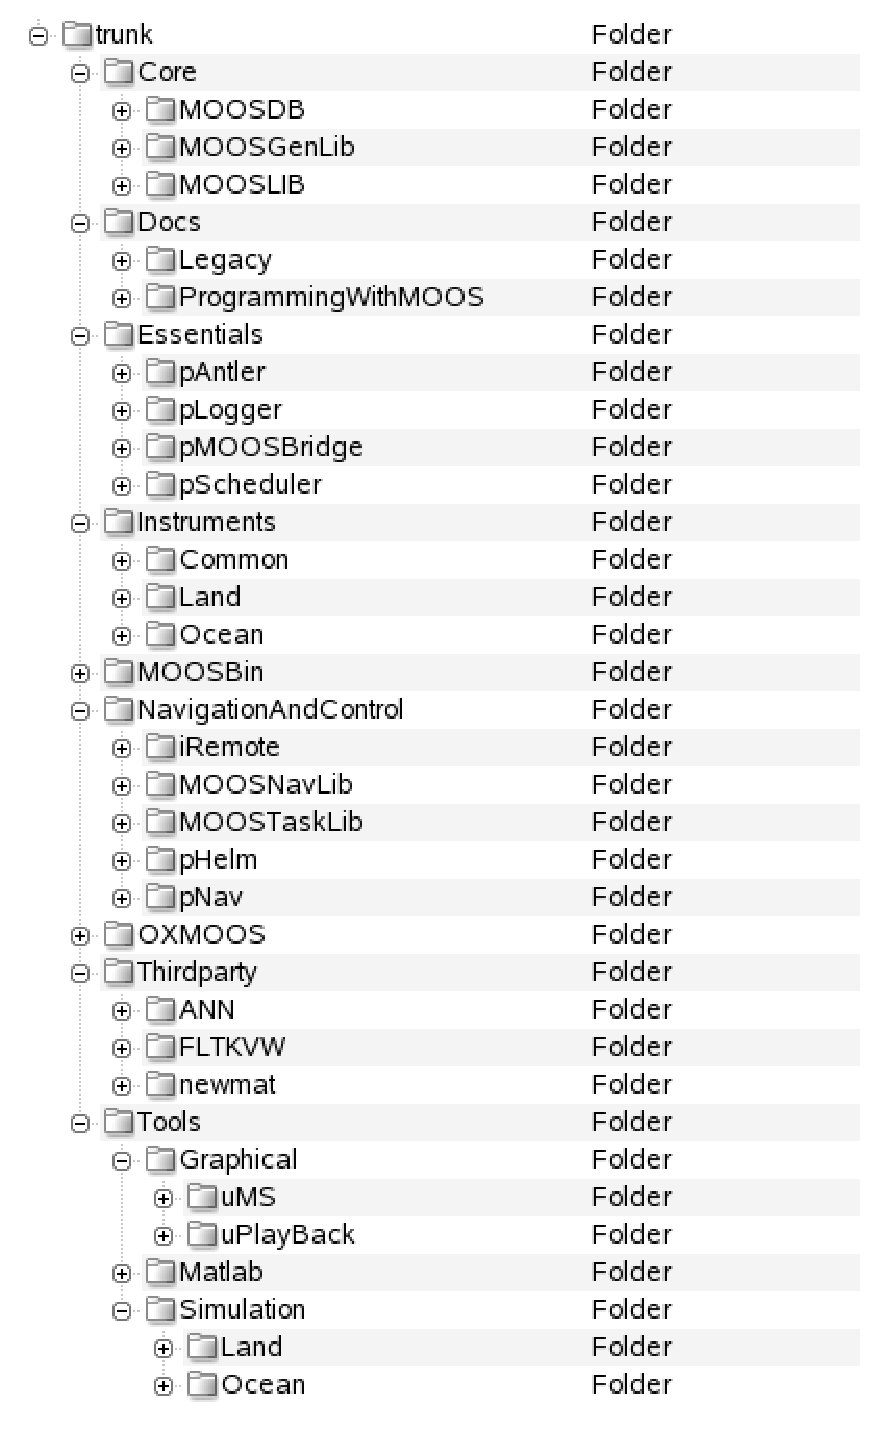
\epsfig{file = ./images/BuildTree.eps , width = 0.9\linewidth}
\caption{The MOOS source tree (as downloaded)}
\end{figure}

Figure \ref{Fig:MOOSTree} shows the shape of the MOOS tree in
release packages.\footnote{You obviously don't have to stick with
this but it has some positives.} In this section we'll survey the contents of each directory. We shall not however describe in any detail what the contents of a directory does when built or how it may be used --- such details can be found elsewhere.

\subsection{Core}

The ``core'' directory contains
code that has nothing per-se to do with robots. It is basically only
concerned with the communications API. See the documentation on Programming with MOOS and
the MOOSComms architecture for more detail. The minimal conceivable build would be these three projects:
the two base MOOS libraries and the MOOSDB server that binds processes
together.


\subsection{Essentials}
This directory also contains domain-neutral applications (i.e.not necessarily only useful for robotics projects) but they are things that tend to be used all the time by folk who have adopted MOOS. It is recommended that you invest time in learning how the processes work -- they'll save you a lot of time.

\subsection{Tools}

The tools subdirectory is again largely domain-independent, but contains, especially in the Graphical subdirectory, some decidedly useful applications.

\subsubsection{Graphical}
Projects in this directory have a dependency on the FLTK cross-platform toolkit. \code{uPlayback} is a lightweight tool which can playback into a MOOS community file created by \code{pLogger}.\code{uMS} is a fantastically useful tool for spying on a multitude of processes talking to each other using the MOOS Communications API.


\subsubsection{Simulation}

This directory contains simulations for ocean- and land-based vehicles. 

\subsection{Matlab}

This directory builds a very useful project. It builds a mexglx or dll file (depending on your OS) which allows Matlab scripts to behave as if they were fully fledged MOOS-enabled processes. It's pretty useful if you want a quick visualisation of data or to prototype some code. To build this project you do need to have Matlab installed.


\subsection{NavigationAndControl}
The \code{NavigationAndControl} directory contains projects that are common
in mobile robotics apps --- \code{pNav} \code{pHelm} and
\code{iRemote}. The former two of these have a dependency on the \code{Newmat} numerical library which can be found in the \code{Thirdparty} directory. There is a case to
put \code{iRemote} in the instruments subfolder as it interfaces to a
``human instrument'' -- but it seemed more robot-centric rather
than sensor-based --- {\it{sub-judice}}.

\subsection{Instruments}

The instruments subtree is pretty obvious -- note that it  includes
\code{iMatlab} which is a peculiar instrument as it provides an
interface to Matlab not a device or human.

\subsection{Thirdparty}

The Thirdparty directory contains code that for the most part is
written by third-party authors. Newmat is a linear algebra package
and FLTKVW is an extension to the FLTK functionality with a few
MOOS-Graphics additions.


\section{Cross-Platform Building using CMake}\label{Sec:UsingCMake}

The use of \code{CMake} allows a code-author to describe in a high-level way what should be built in a project. The important point
from this is that it allows (via ``meta-make'' files called
\code{CMakeLists.txt} found in every directory) Make files to be
written for Unix and Microsoft developer studio development alike.
This is a massive win in terms of cross-platform development /
project management. \footnote{Of course if one only develops for
one OS it is hard to see the benefit.}


By toggling the relevant fields in the ccmake curses-GUI you can
turn on/off Makefile generation for different parts of the project.
Pressing ``c'' to configure then parses the newly included
CMakeLists.txt files and may present some new options for you to
select. A basic build should work out-of-the-box simply by accepting the default values.  But to be sure we'll now walk through the process step by step.

\begin{enumerate}
\item  Download and install \code{CMake} for your platform (from
\url{www.cmake.org or} the MOOS website).
%
\item ``cd'' into the MOOS root directory.
%
\item Type \code{ccmake ./}  -- you should see
something like Figure \ref{Fig:CMake1}.
\begin{figure}[ht]\label{Fig:CMake1}
\centering 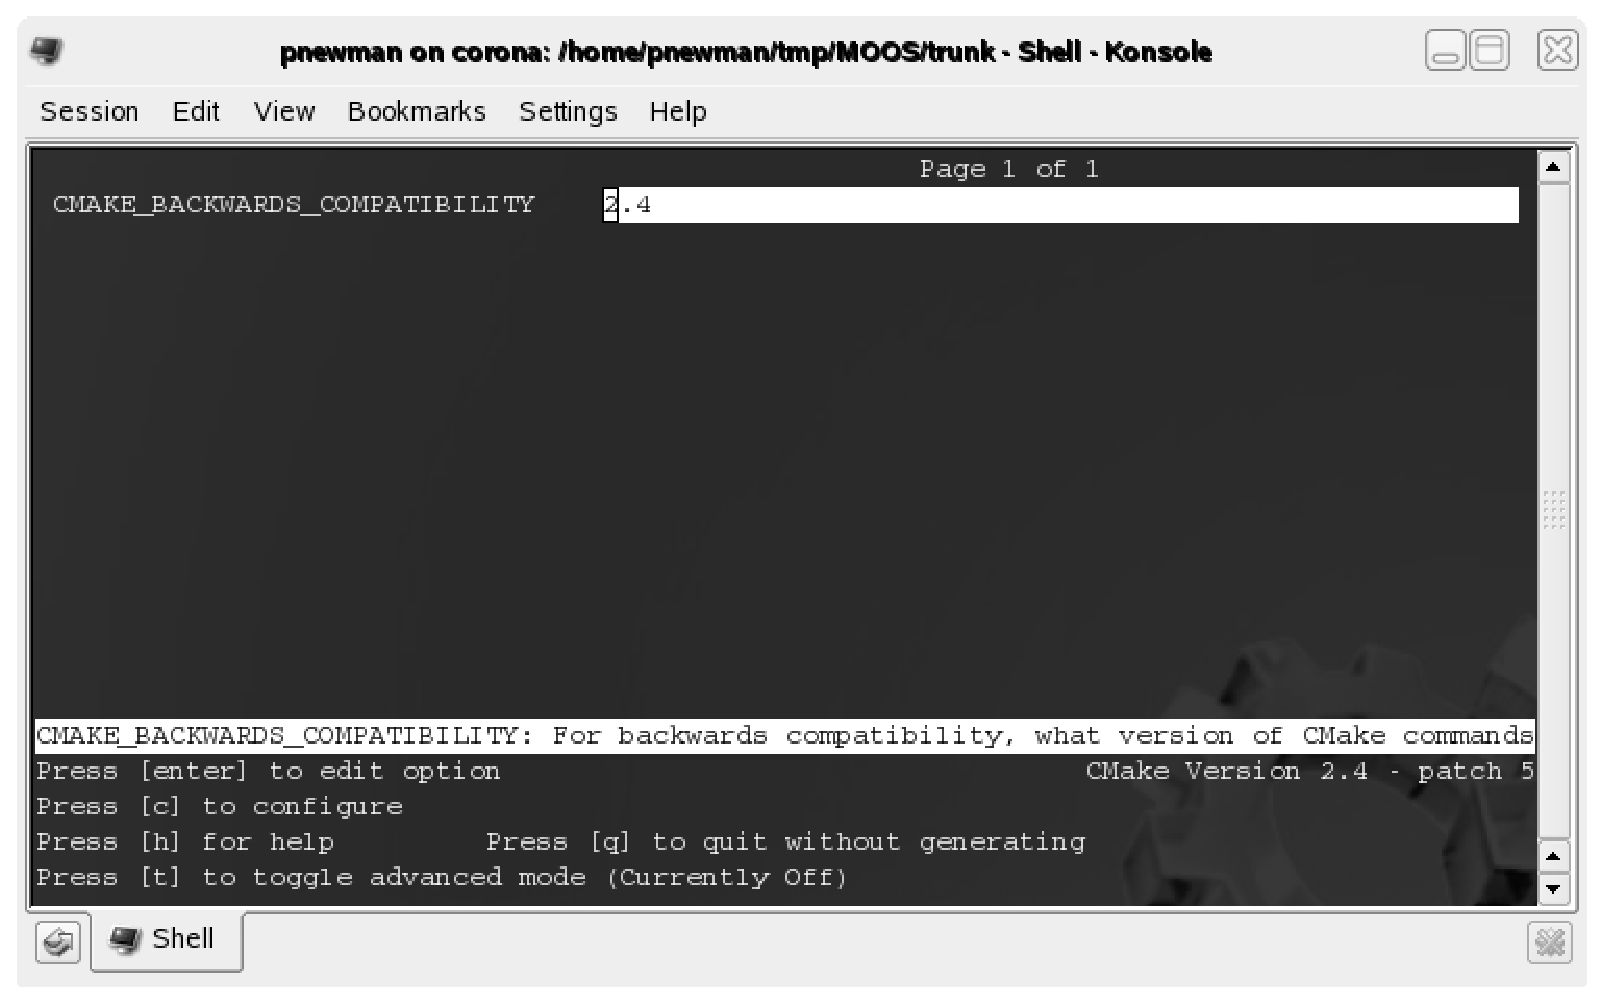
\epsfig{file = ./images/CMakeSteps/CMake1.eps , width =  \linewidth}
\caption{The initial CMake Screen - Win32 platforms have a
gui-dialog rather than an ncurses interface}
\end{figure}
%
\item Press ``c'' to configure -- the screen should look like
something like Figure \ref{Fig:CMake2}.
\begin{figure}[ht]\label{Fig:CMake2}
\centering 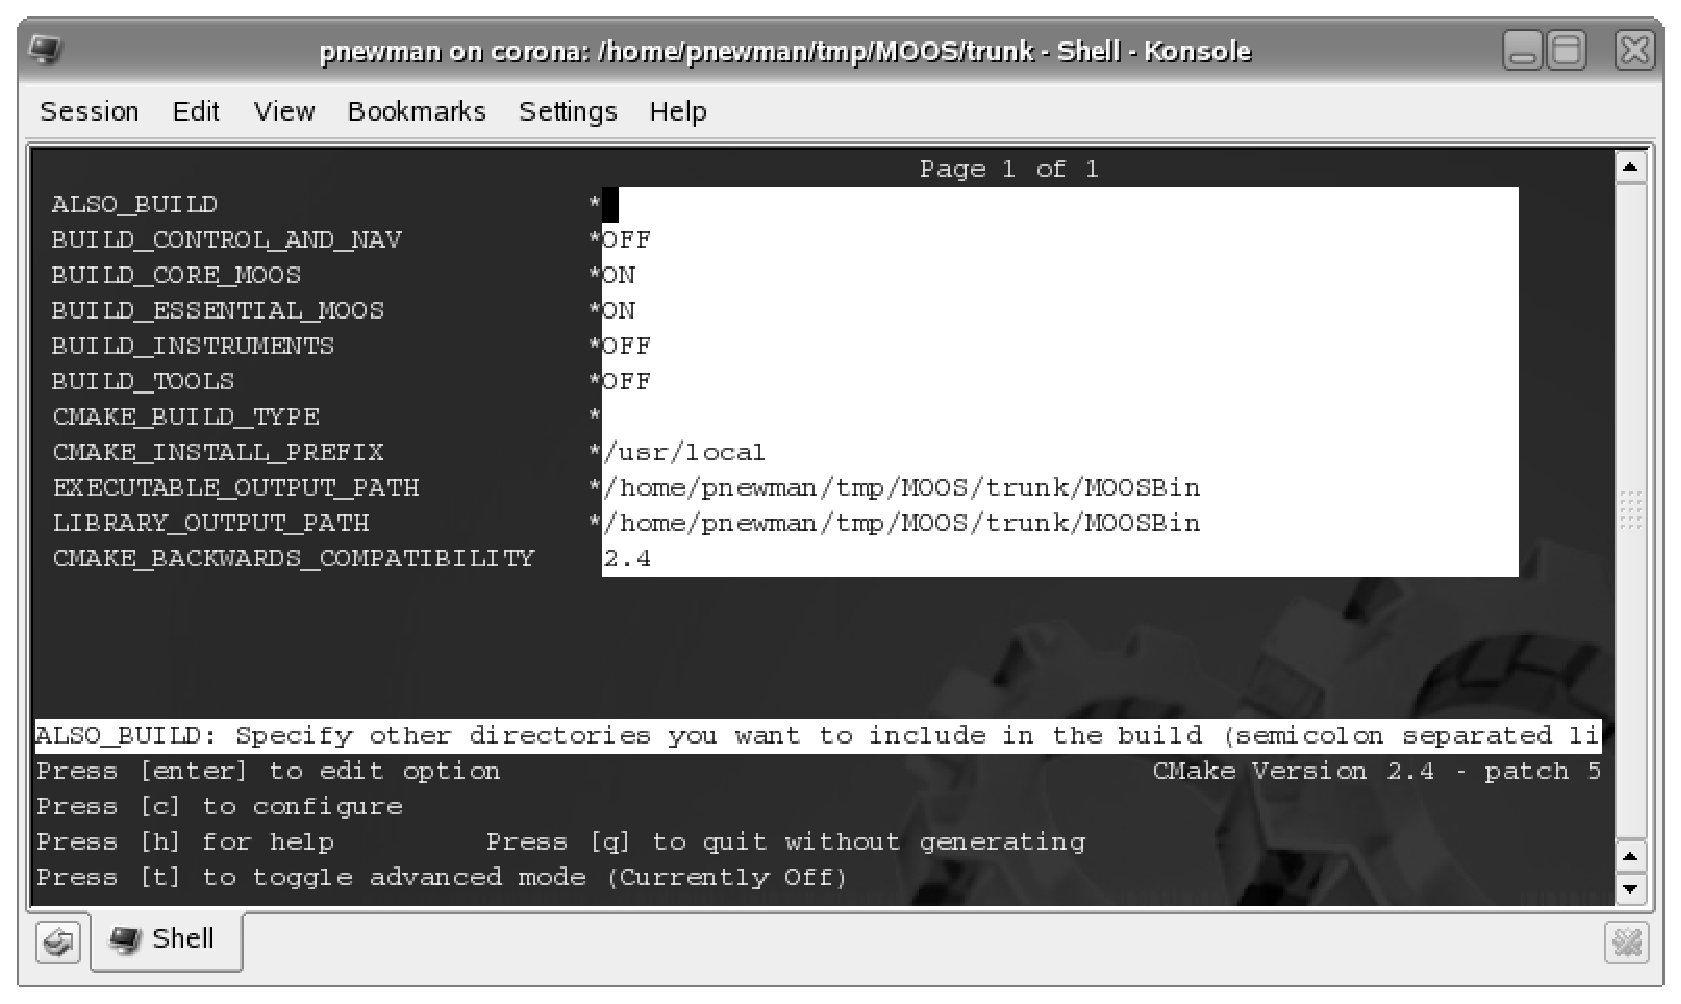
\epsfig{file = ./images/CMakeSteps/CMake2.eps , width = \linewidth}
\caption{The initial CMake Screen after an initial configure --
note no option to generate Make files is present as yet. Build
directories and build options (i.e. what to build and what not) can
be selected at this stage. }
\end{figure}
*
\item Press ``c'' to configure once more. The screen should now look
something like  Figure \ref{Fig:CMake3}.
\begin{figure}[ht]\label{Fig:CMake3}
\centering 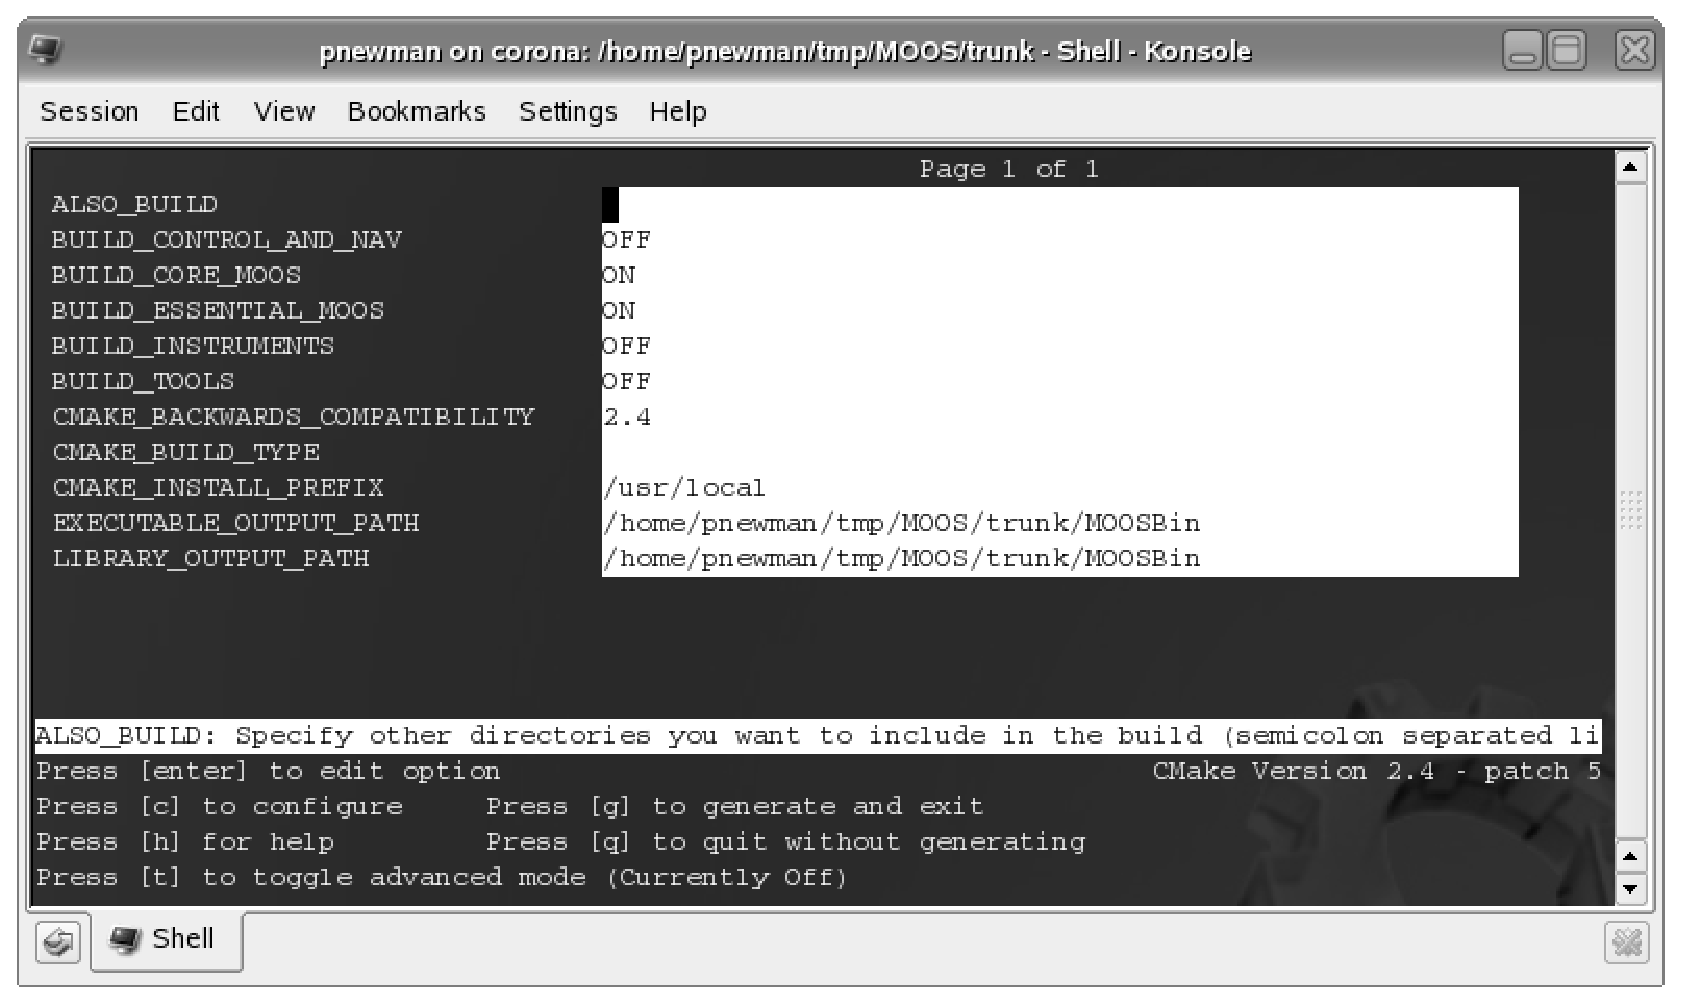
\epsfig{file = ./images/CMakeSteps/CMake3.eps , width = \linewidth}
\caption{The final CMake Screen before generating the build files
(``.dsp'' or Makefile --- depending on platform). Please note
``Configure'' may have been selected several times before this
final option is presented. }
\end{figure}
%
\item Notice an option ``g'' has appeared saying we are good to
go....Press ``g'' to generate the MOOS make files. If you have
followed the above steps CMake will exit and you'll see (along
with one or two other CMake generated files) a master Makefile (or dsp/dsw/sln file for DevStudio builds) in
the root directory.
\item You are now ready to build the project. If you have selected an IDE build, (like Devstudio or KDevelop) load the relevant newly created project file into your idea and perform whatever steps are needed to build. In Figure \ref{Fig:CMake4} I've just typed ``make'' in a linux
terminal. I went with all the default options and now just ``Core'' and ``Essential'' projects are being built. I have a warm fuzzy about this.
\begin{figure}[ht]\label{Fig:CMake4}
\centering 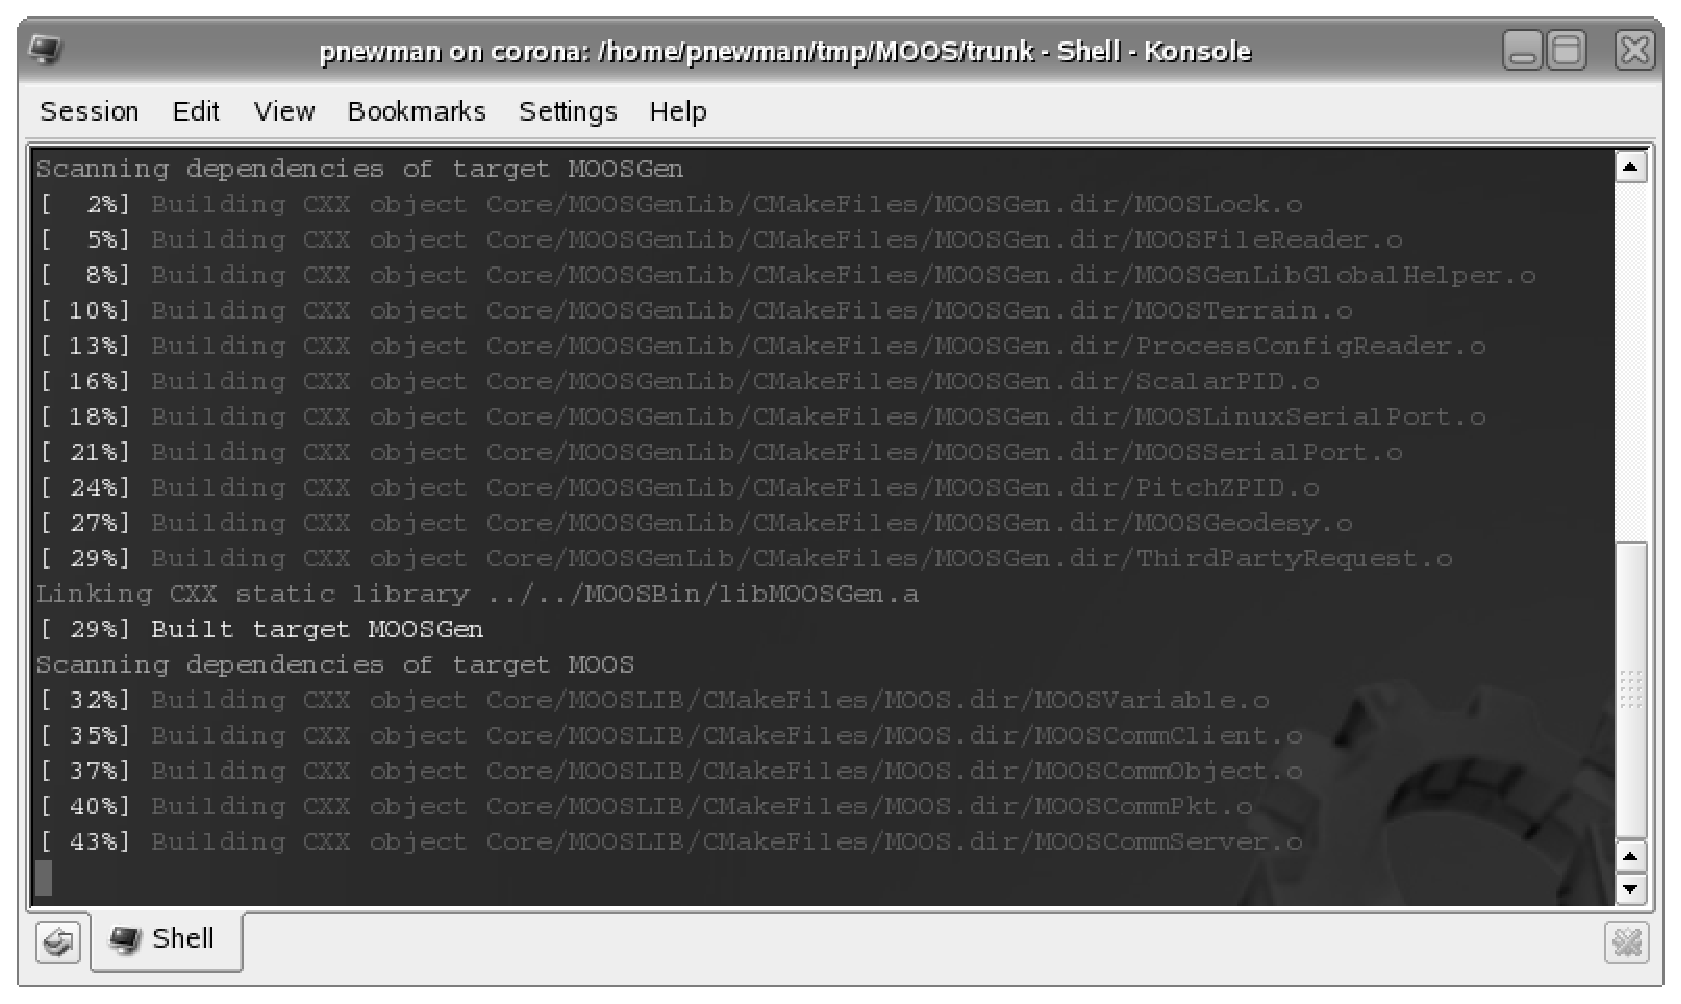
\epsfig{file = ./images/CMakeSteps/CMake4.eps , width = \linewidth}
\caption{CMake has made the project files (which for me today in this example is a Linux ``Makefile'') and exited. Having typed ``make'' the build proceeds. The executables will be placed in the \code{MOOSBin} directory. }
\end{figure}

\end{enumerate}



Note that the Utils directory includes massively useful GUI
applications which link against FLTK. You are expected to have the
library and include files in your system path (this should have
been done for you using the {\it{configure, make, make install}} paradigm
when building the FLTK library)



\subsection{Incorporating Private Subtrees}\label{Sec:PrivatCode}

Entering a suitable directory or symbolic link in the
\code{ALSO\_BUILD} field causes CMake to recurse into that
directory when creating Make files. This way developers can
include their own projects in the build paradigm. For example, the
Oxford Mobile Robotics group has a directory called OXMOOS which
lives in a directory in MOOS (just like Core or Utils does).
Typing OXMOOS in the \code{ALSO\_BUILD} field causes CMake to
recurse into the OXMOOS directory and follow the instructions in
the CMakeLists.txt file therein (which causes it to recurse
further down into each of our individual application projects).
The advantage of this is that it inherits all the build flags and library
settings of the parent MOOS project, and so things like the library
paths (MOOSBin in the example above) are automatically passed to
the compiler.\\

\subsection{Where are the Binaries?}
By default binaries and
libraries are placed in \code{\textit{root}/MOOSBin}. This of course can be
changed simply by typing in your preferred destination during the
build system set up using CMake.\footnote{Devstudio users will
find the binaries in debug/release/releasewithdebug directories
within MOOSBin depending on the active project configuration
selected in the IDE.} See Figure \ref{Fig:CMake2}.


\section{Living Without CMake}\label{Sec:RollYourOwn}

Some MOOS users may not wish to use the CMake infrastructure  (a
CMakeLists.txt file in each directory) or tree provided in the
releases -- preferring instead to use old trusted Make files they have
written themselves for whatever platform they wish to
develop/deploy on. This of course will work --- the source in no
way depends upon the build system.
If this is your preferred method, then you will need to know which
include paths are required and what libraries must be linked against.

\subsection{Include Paths}
To compile an application that uses the MOOS Comms API you need to
add the following include paths.

\begin{center}
\begin{description}
\item \code{\textit{root}/Core/}
\end{description}
\end{center}
Please note, header files are included relative to the
\code{\textit{root}/Core} directory for example by using \verb!#include<MOOSLIB/MOOSCommsCLient.h>!

\subsection{Library Paths}
To link an application that uses the MOOS Comms API you need to
add the following library paths
\begin{description}
\item \code{\textit{root}/MOOSBin} \footnote{Windows users -- note Devstudio further qualifies this path with ``Debug'' or ``Release'' etc subdirectories}
\end{description}
For historical reasons all binaries including libraries are placed
in the \code{\textbf{MOOSBin}} directory \footnote{This is something that needs
looking at  with separate \code{lib} and \code{bin} directories being preferable and
planned.}. You will also need to link against the libraries stated
in Section \ref{Sec:Libs}.

\subsection{Libraries to Link Against}\label{Sec:Libs}
To build an application that uses the core MOOS libraries, you will need to link against the following libraries (listed by OS).
\begin{center}
% use packages: array
\begin{tabular}{lll}
\textbf{Windows} & \textbf{Linux} & \textbf{Solaris} \\
wsock32.lib & libm.a & libm.a \\
comctl32.lib & libpthread.a & libpthread.a \\
MOOS.lib & libMOOS.a & libsocket.a \\
MOOSGen.lib & libMOOSGen.a & libnsl.a \\
\textit{(console libs)} & × & libMOOS.a \\
× & × & libMOOSGen.a
\end{tabular}
\end{center}

If you want to roll your own Make files for the graphical applications inside the MOOS tree, look at the \code{CMakeLists.txt} files in the top root directory and the individual application directories to see what additional libraries are required.


\end{document}
